\chapter{提案システム}

\thispagestyle{myheadings}

\section{はじめに}
本章では,運動教室で実施される集団でのコグニサイズにおいて,認知課題の負荷を個別に調整可能なシステムを提案する.本稿では,コグニサイズの一つであるコグニステップに対応した提案システムを開発する.提案システムでは,コグニステップの認知課題の正答率を蓄積し,蓄積した認知課題の正答率に応じて認知課題の負荷を個別に調整する.次節以降に提案システムの概要,処理の流れについて述べる.

\if0
本章では,ベッド型の下肢リハビリを拡張する,下肢リハビリへのモチベーションを向上させるための没入型歩行感覚提示システムについて述べる.提案システムは没入感が高を高めるため,現実的な3DCGを利用し実現する.センサが内蔵されたHMDを使用することで,リハビリ患者の頭部の動きに追従した映像提示により,没入感が高まることが期待できる.次節以降に提案システムの概要,処理の流れについて述べる.
\fi

\section{コグニステップ}
1.1節で示したとおり,コグニステップは数字を数えながら左右の足で交互にステップをする運動と同時に,一定間隔ごとの決められた数字で拍手をする認知課題を行う.文献\cite{認知症予防へ向けた運動コグニサイズ}では,拍手をする数字の間隔を変更することで認知課題の負荷を調整可能としている.

\section{提案システムの概要}
提案システムでは,身体動作の認識が可能なKinectを使用し,コグニステップの認知課題の拍手動作を検出する.検出した拍手動作を利用し,認知課題の正誤判定を行う.コグニステップ実施中は認知課題の正誤判定を集計し,コグニステップ終了後に正誤判定の集計結果から認知課題の正答率を算出し,データベースに蓄積する.提案システムの構成図を図\ref{fig:system}に示す.認知課題の視覚的フィードバックを行うため,Kinectに内蔵されるRGBカメラで参加者を撮影し,撮影した動画を参加者の正面にプロジェクタで投影する.プロジェクタの投影面には図\ref{fig:vm_init}の赤枠内に示すように,認知課題を個別に表示する.表示する認知課題の負荷はPC上の管理画面で変更可能である.図\ref{fig:db_init}にPC上の管理画面を示す.データベースに蓄積した認知課題の正答率をPC上の管理画面で参照し,認知課題の正答率に応じて認知課題の負荷を個別に調整する.次節以降にそれぞれの処理について述べる.

\begin{figure}[tbp]
	\centering
			\includegraphics[width=0.9\textwidth]{chap2-figure/system.eps}
	\caption{システム構成図}
	\label{fig:system}
\end{figure}

\if0
\begin{figure}[tbp]
	\centering
			\includegraphics[width=0.6\textwidth]{chap2-figure/kinect.eps}
	\caption{Kinect}
	\label{fig:kinect}
\end{figure}
\fi

\begin{figure}[tbp]
	\centering
			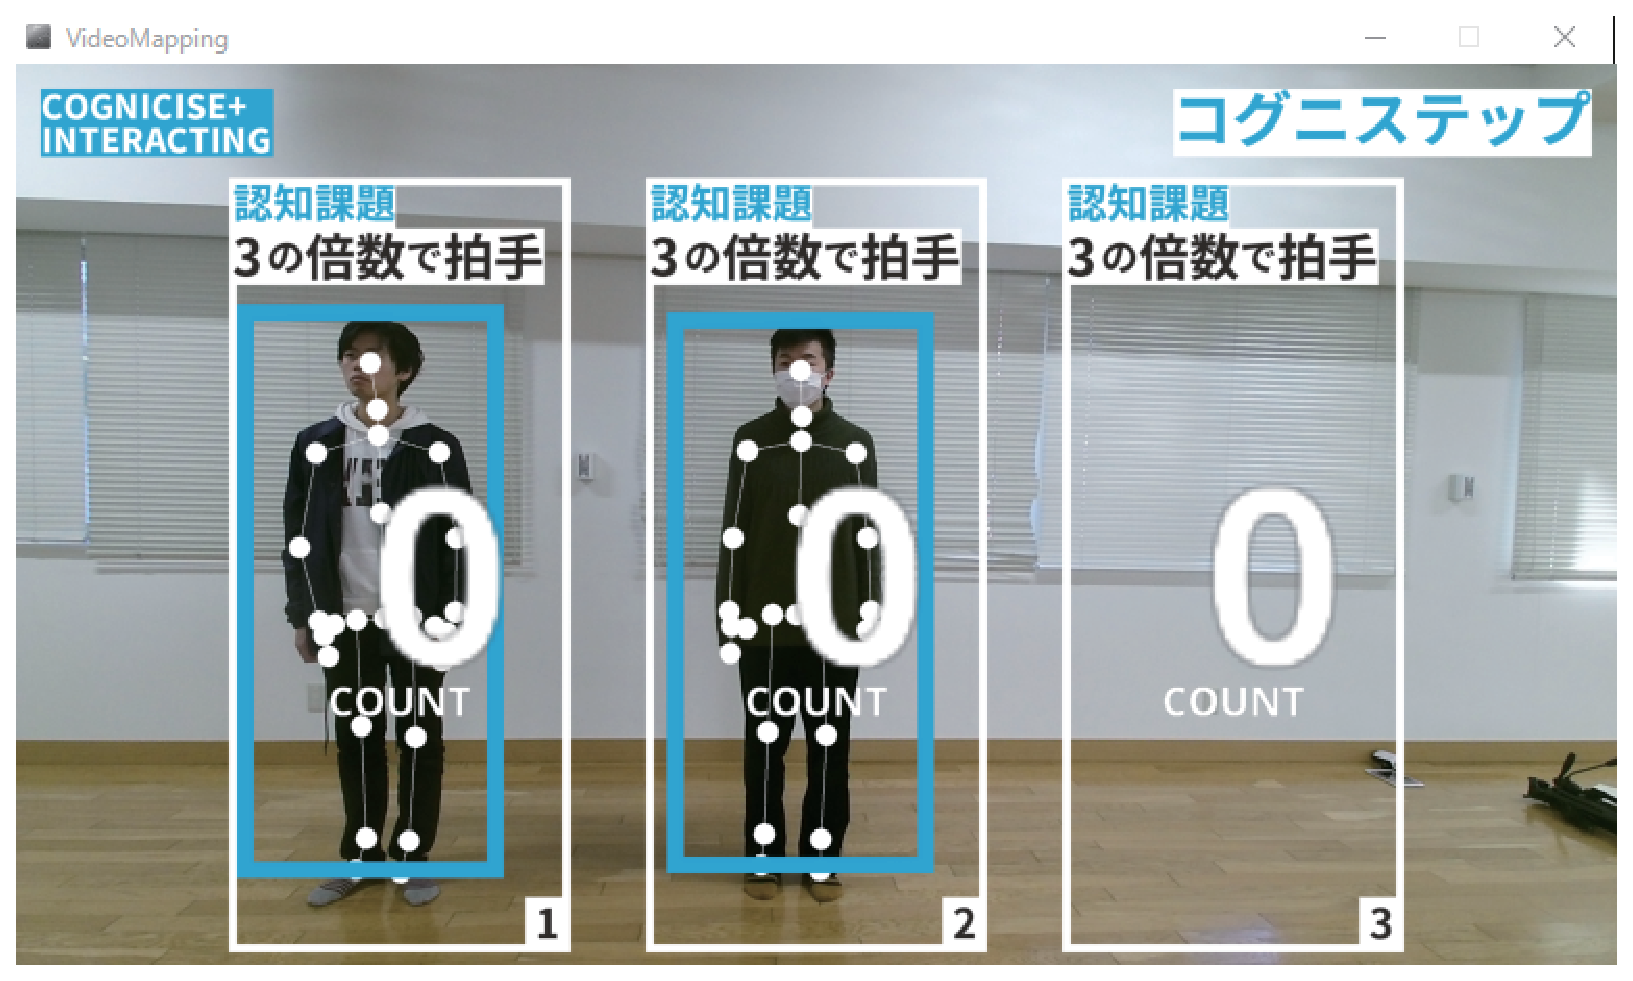
\includegraphics[width=0.9\textwidth]{chap2-figure/vm_init.eps}
	\caption{プロジェクタ投影面}
	\label{fig:vm_init}
\end{figure}

\begin{figure}[tbp]
	\centering
			\includegraphics[width=0.9\textwidth]{chap2-figure/db_init.eps}
	\caption{PC上のシステムの管理画面}
	\label{fig:db_init}
\end{figure}


\if0
提案システムでは,ベッド型の下肢リハビリ装置の下肢可動部にKinectV2\cite{KinectV2}を置き,歩行の検出を行う.KinectV2を図\ref{fig:kinect}に示す.KinectV2をセンサとして使用する.提案システムの歩行の検出にKinectV2を使用したシステム構成を図\ref{fig:beforesystemarc}に示す.ベッド型の下肢リハビリ装置の下肢部分の手前にKinectV2を設置する.処理の流れを図\ref{fig:片桐1}に示す.KinectV2からの取得した映像を二値化行い,図\ref{fig:kinectsystemarc}に示す,ベッド型の下肢リハビリ装置の下肢可動部の検出を行う.図\ref{fig:kinectsystemarc}に示す矩形の重心点の座標を取得し閾値を設定し,歩行判定を行う.歩行判定を基にキャラクタは歩行動作を行う.

\begin{figure}[tbp]
	\centering
			\includegraphics[width=0.8\textwidth,angle = 270]{chap2-figure/kinect.eps}
	\caption{KinectV2}
	\label{fig:kinect}
\end{figure}

\begin{figure}[tbp]
	\centering
			\includegraphics[width=0.8\textwidth]{chap2-figure/beforesystem.eps}
	\caption{KinectV2を使用したシステム構成図}
	\label{fig:beforesystemarc}
\end{figure}

\begin{figure}[tbp]
	\centering
			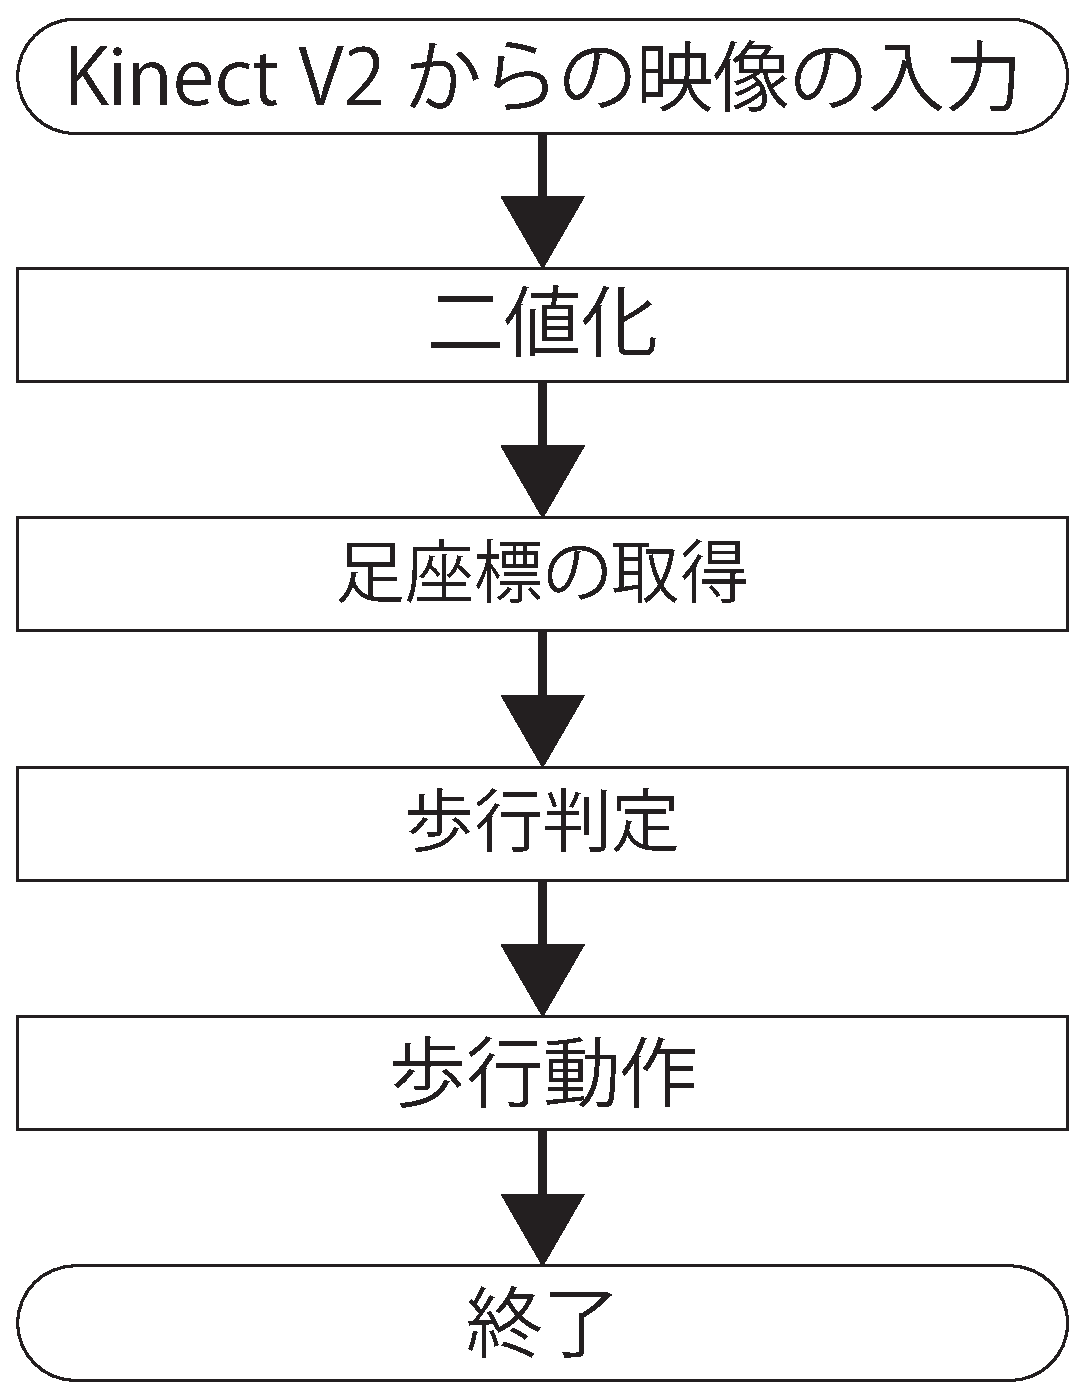
\includegraphics[width=0.3\textwidth]{chap2-figure/katagiri1.eps}
	\caption{処理の流れ}
	\label{fig:片桐1}
\end{figure}

\begin{figure}[tbp]
	\centering
			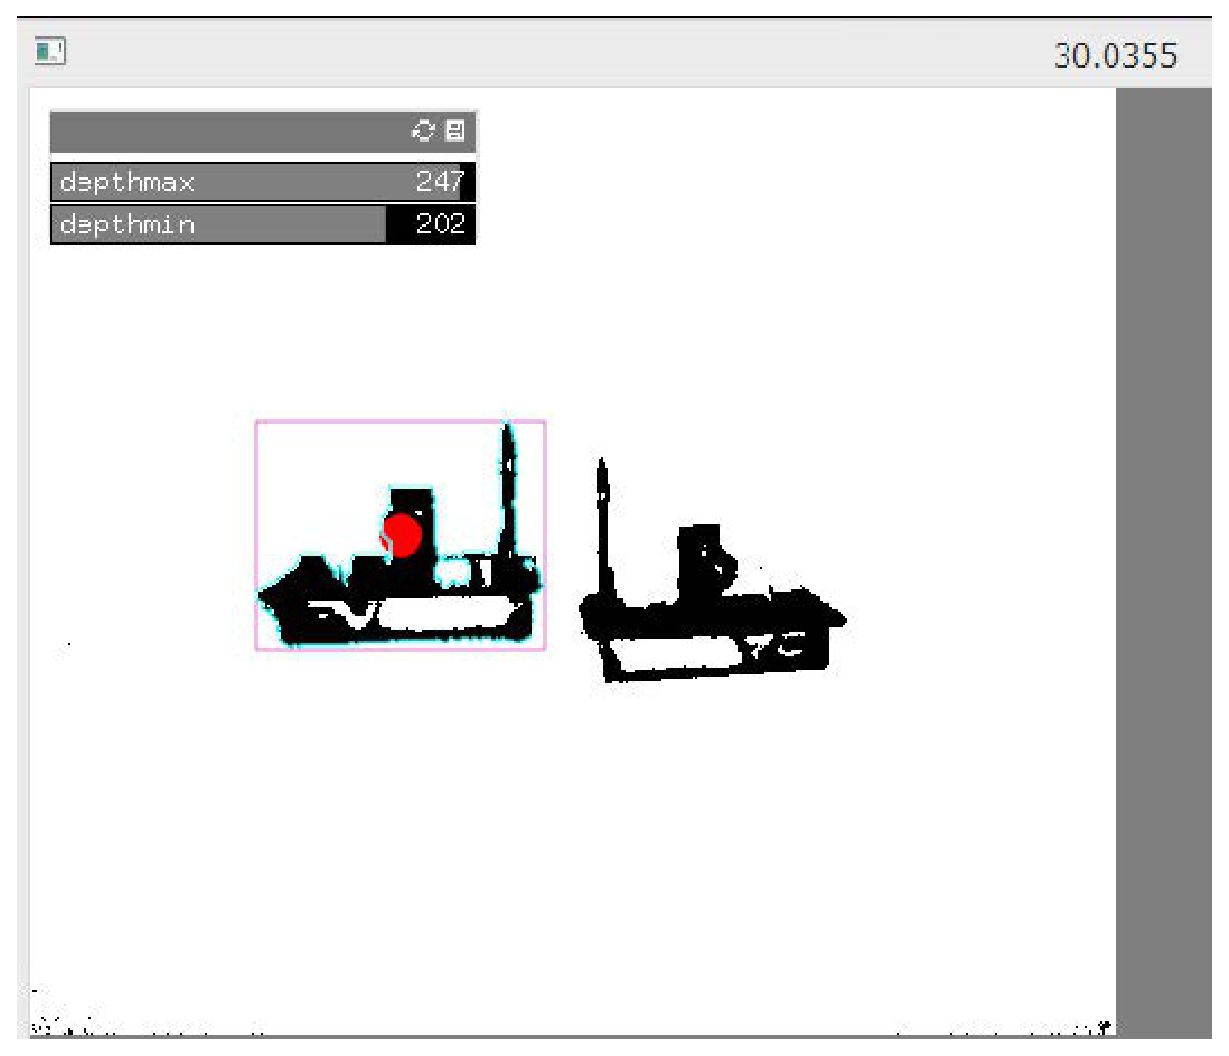
\includegraphics[width=0.8\textwidth]{chap2-figure/kinectsystem.eps}
	\caption{KinectV2の検出画像}
	\label{fig:kinectsystemarc}
\end{figure}
\fi

\section{処理の流れ}

\begin{figure}[tbp]
	\centering
			\includegraphics[width=0.9\textwidth]{chap2-figure/db_management_user.eps}
	\caption{参加者の管理画面}
	\label{fig:db_management_user}
\end{figure}

\begin{figure}[tbp]
	\centering
			\includegraphics[width=0.9\textwidth]{chap2-figure/db_regist_new_user.eps}
	\caption{新規参加者の登録画面}
	\label{fig:db_regist_new_user}
\end{figure}

\begin{figure}[tbp]
	\centering
			\includegraphics[width=0.9\textwidth]{chap2-figure/db_select_user.eps}
	\caption{参加者の選択画面}
	\label{fig:db_select_user}
\end{figure}

\begin{figure}[tbp]
	\centering
			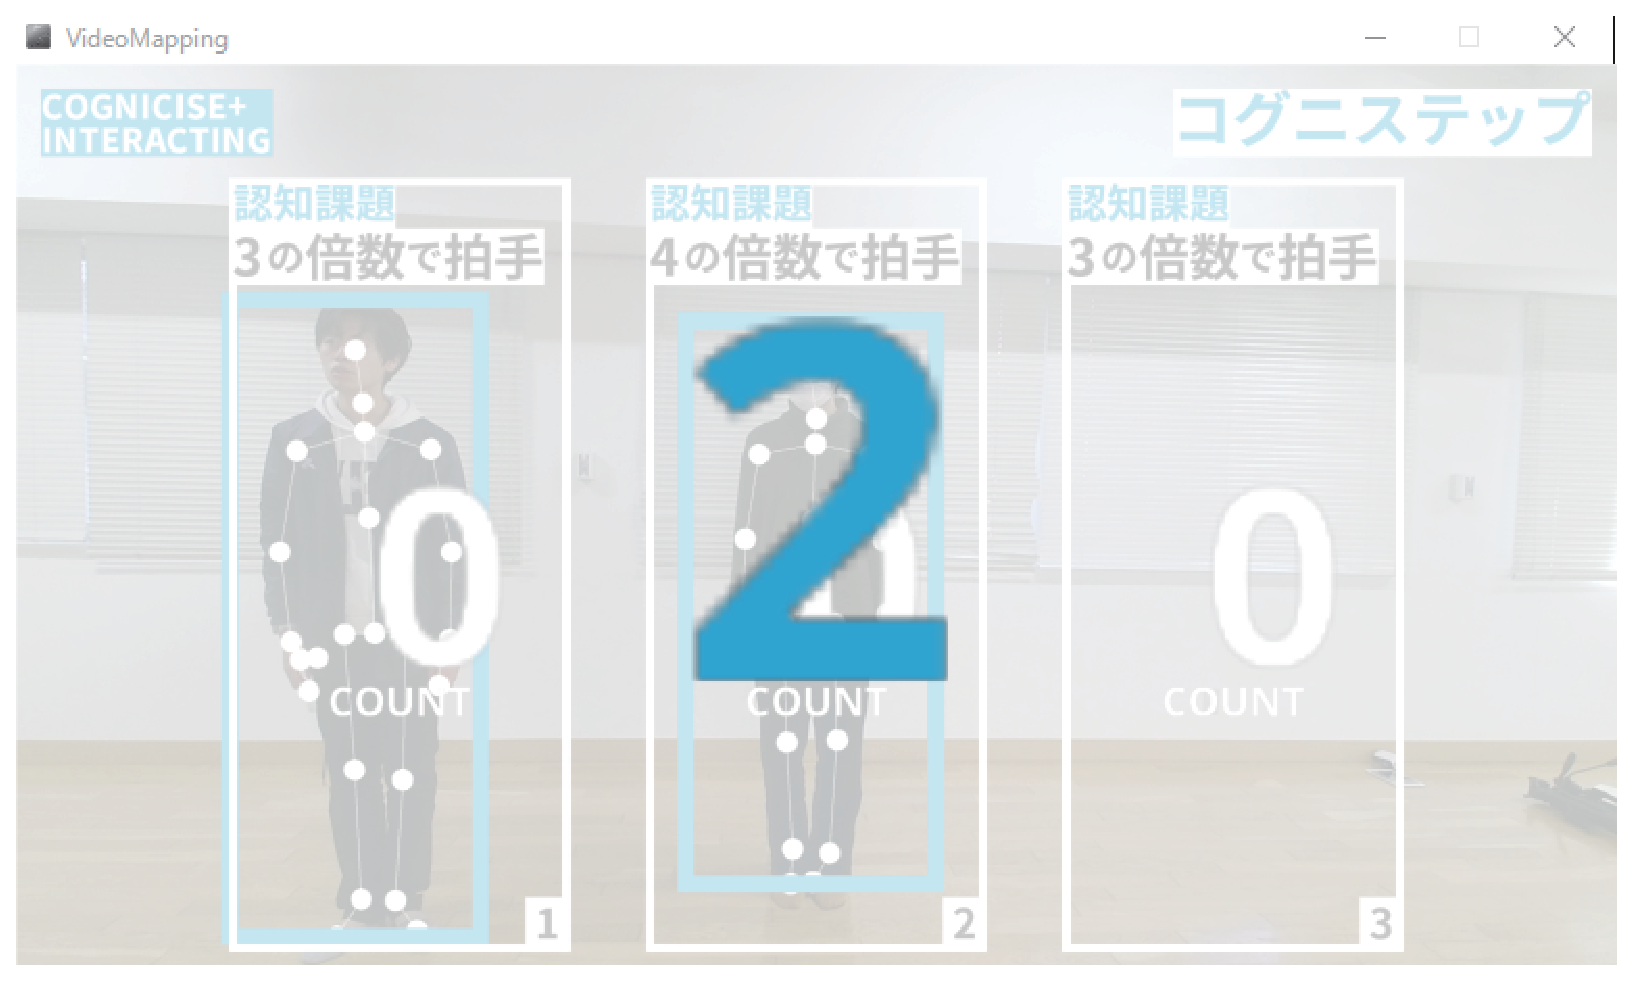
\includegraphics[width=0.9\textwidth]{chap2-figure/vm_start.eps}
	\caption{プロジェクタ投影面(開始時)}
	\label{fig:vm_start}
\end{figure}

\begin{figure}[tbp]
	\centering
			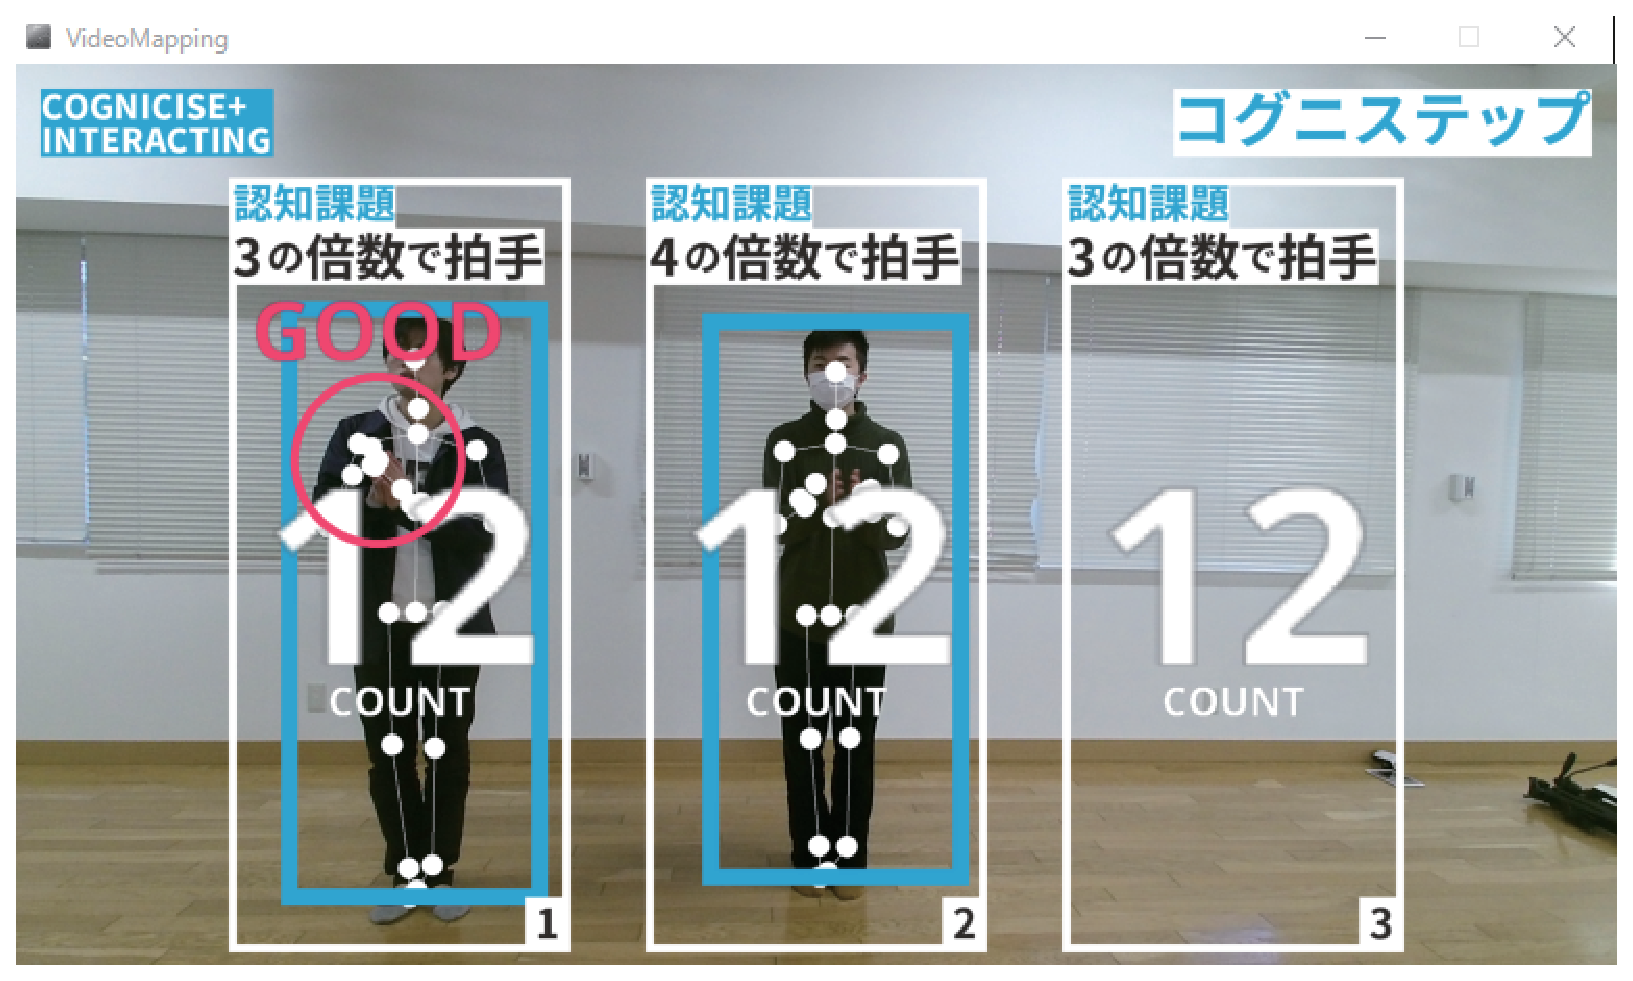
\includegraphics[width=0.9\textwidth]{chap2-figure/vm_clap.eps}
	\caption{プロジェクタ投影面(認知課題の正答時)}
	\label{fig:vm_clap}
\end{figure}

\begin{figure}[tbp]
	\centering
			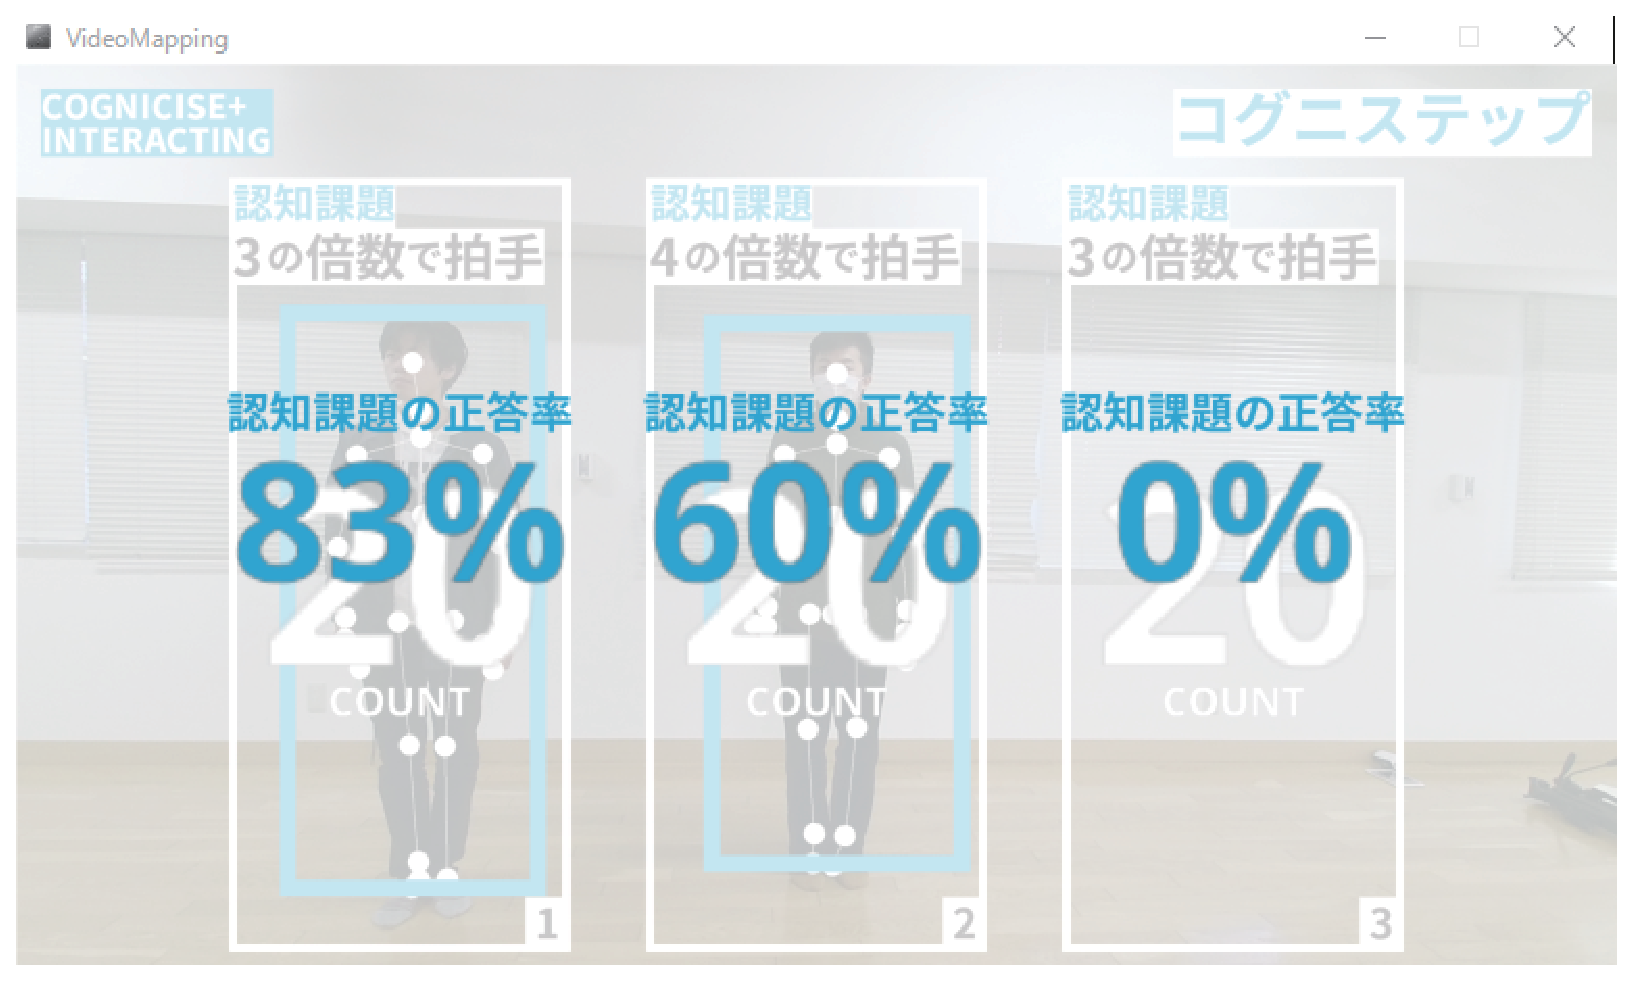
\includegraphics[width=0.9\textwidth]{chap2-figure/vm_answer_rate.eps}
	\caption{プロジェクタ投影面(認知課題の正答率の表示)}
	\label{fig:vm_answer_rate}
\end{figure}

\begin{figure}[tbp]
	\centering
			\includegraphics[width=0.9\textwidth]{chap2-figure/db_user_info.eps}
	\caption{参加者情報画面}
	\label{fig:db_user_info}
\end{figure}

\begin{figure}[tbp]
	\centering
			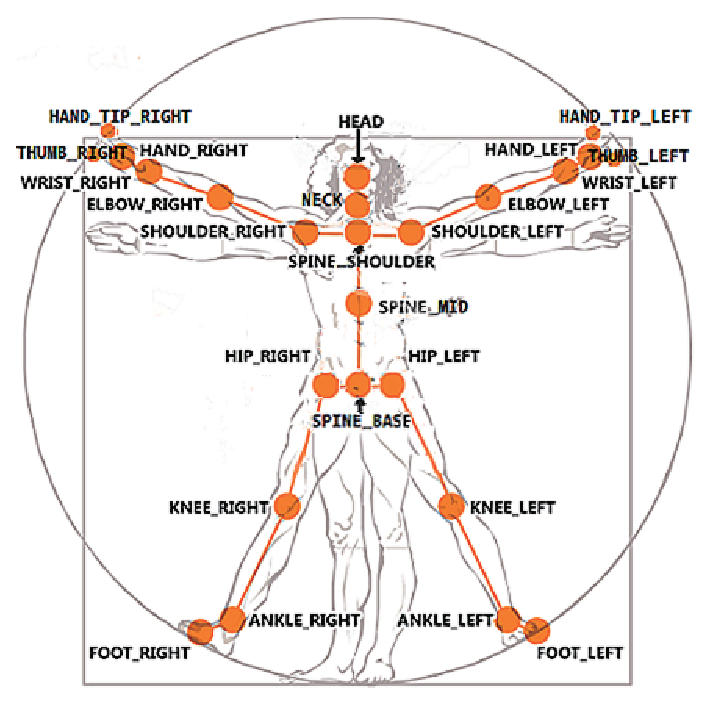
\includegraphics[width=0.7\textwidth]{chap2-figure/skelton_position.eps}
	\caption{Skeleton positions relative to the human body}
	\label{fig:skelton_position}
\end{figure}

\if0
提案システムの処理の流れについて述べる.処理の流れを図\ref{fig:片桐2}に示す.
提案システムの開始方法は,HMDをつなげたPCのマウスを左クリック又はキーボードのスペースキーで開始される.HMDに提示される開始画面を図\ref{fig:start}に示す.開始後,キャラクタの一人称視点の映像が提示され歩行が開始される.開始後の画面を図\ref{fig:gemestart}に示す.患者は設定時間が終了するまで下肢リハビリを続ける.設定した時間が終了すると,図\ref{fig:end}の画面が提示される.
\begin{figure}[tbp]
	\centering
			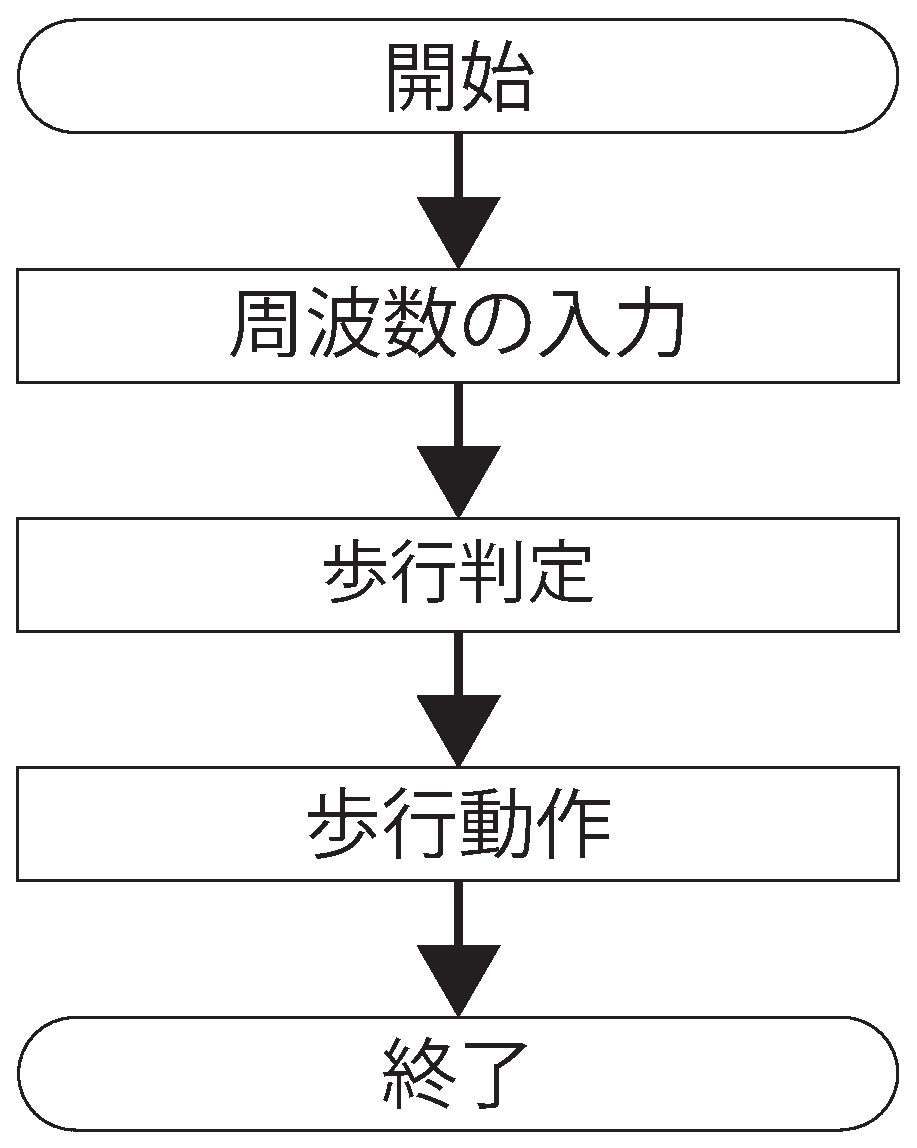
\includegraphics[width=0.3\textwidth]{chap2-figure/katagiri2.eps}
	\caption{処理の流れ}
	\label{fig:片桐2}
\end{figure}

\begin{figure}[tbp]
	\centering
			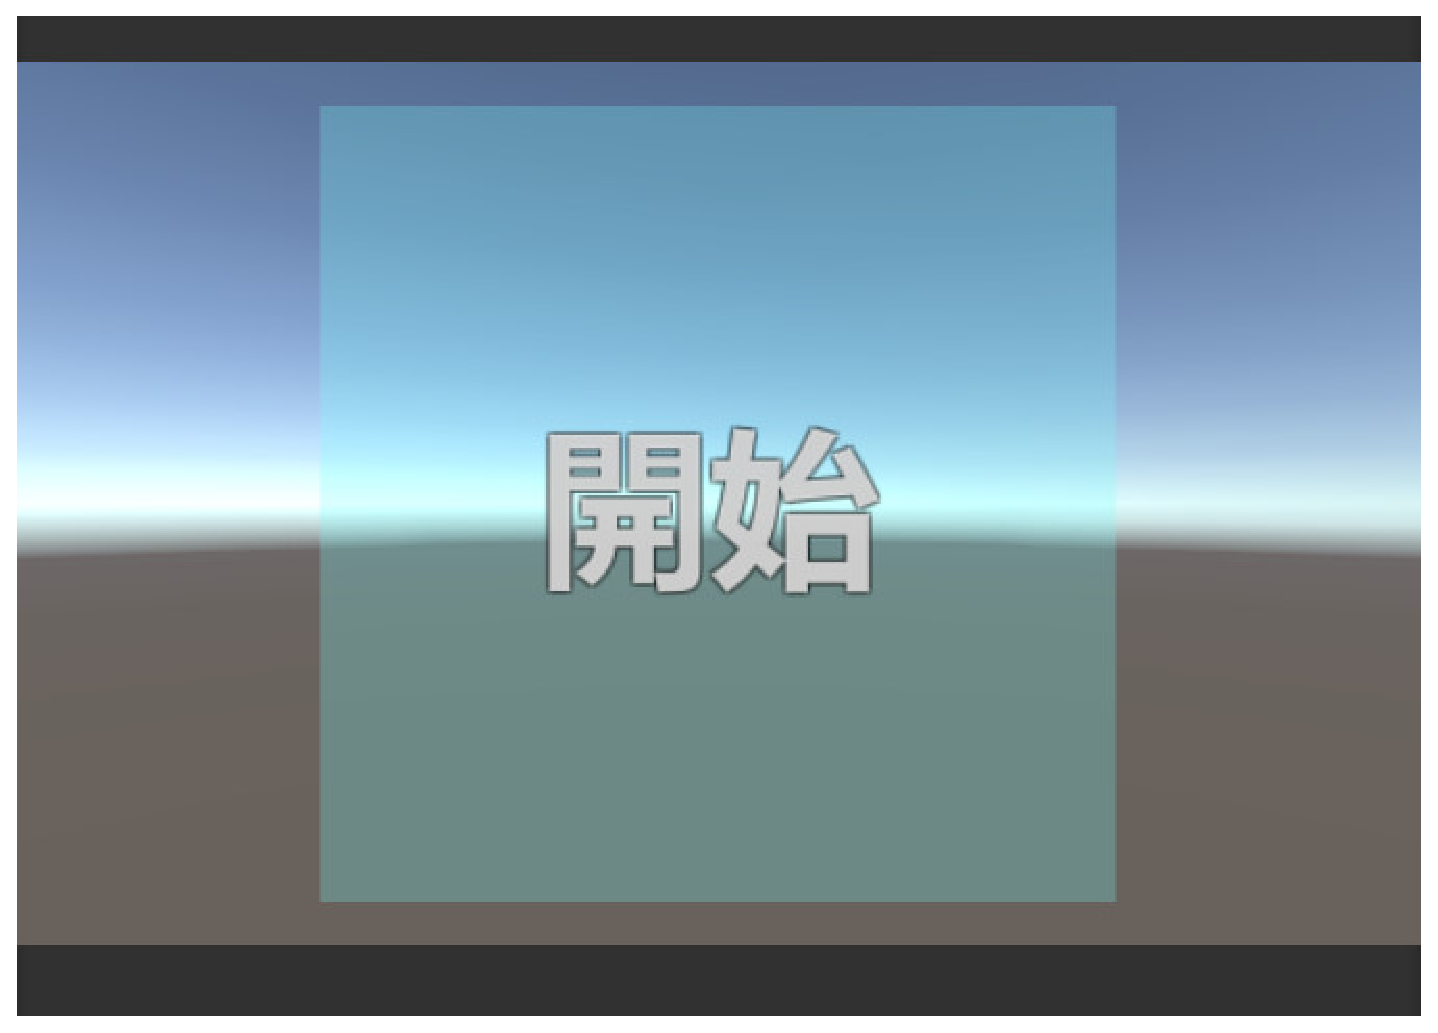
\includegraphics[width=0.9\textwidth]{chap2-figure/start.eps}
	\caption{スタート画面}
	\label{fig:start}
\end{figure}

\begin{figure}[tbp]
	\centering
			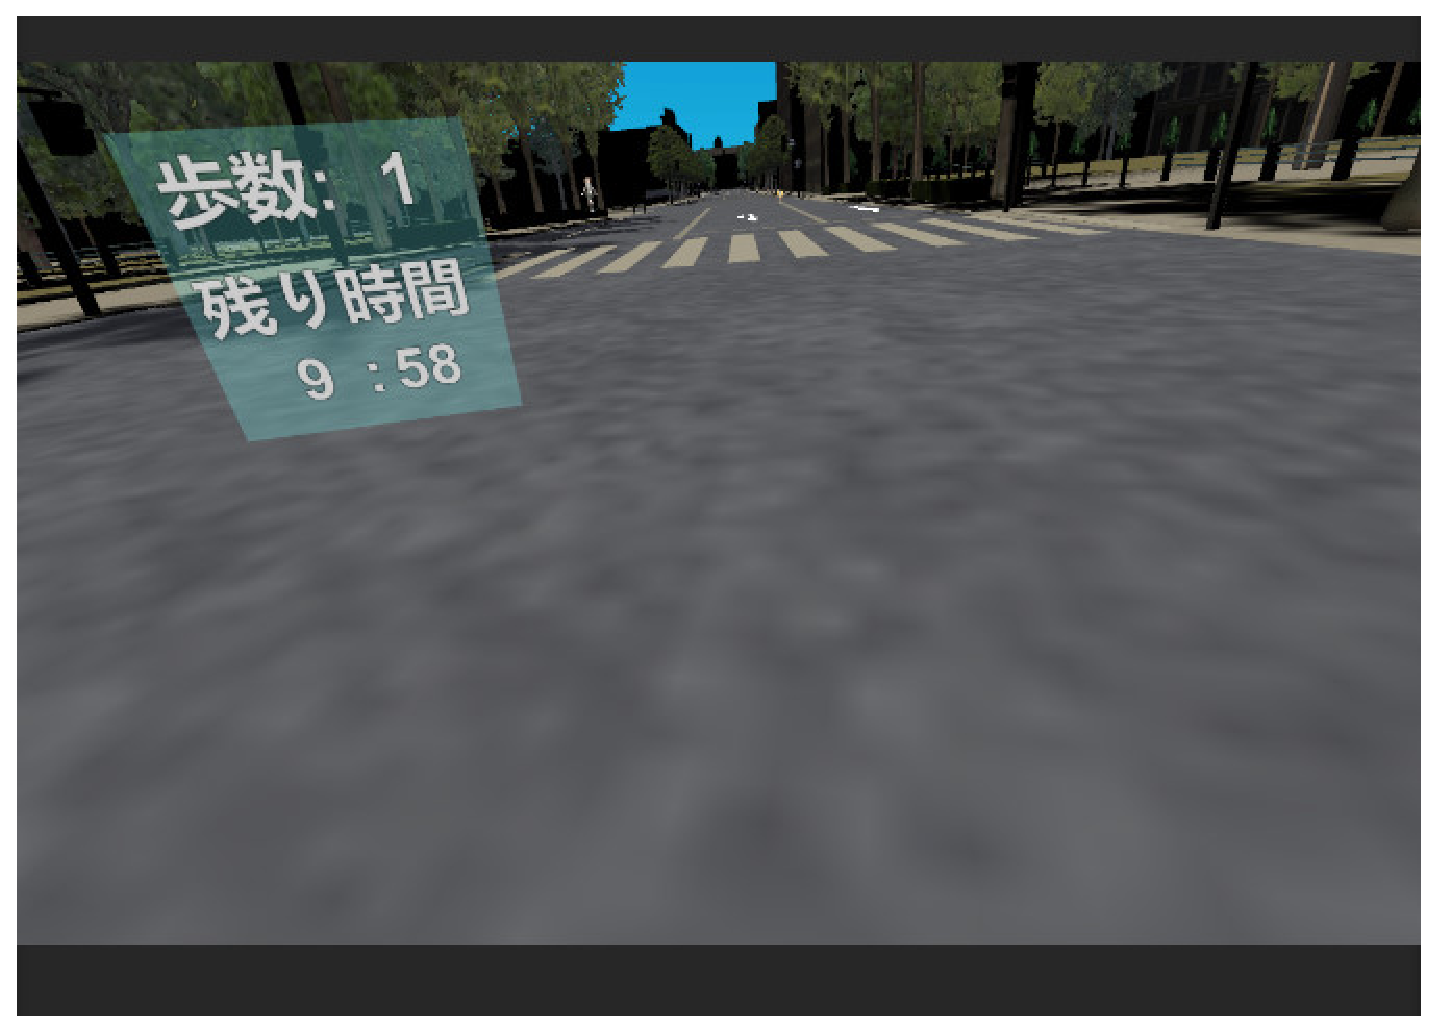
\includegraphics[width=0.9\textwidth]{chap2-figure/midstream-1.eps}
	\caption{開始後画面}
	\label{fig:gemestart}
\end{figure}

\begin{figure}[tbp]
	\centering
			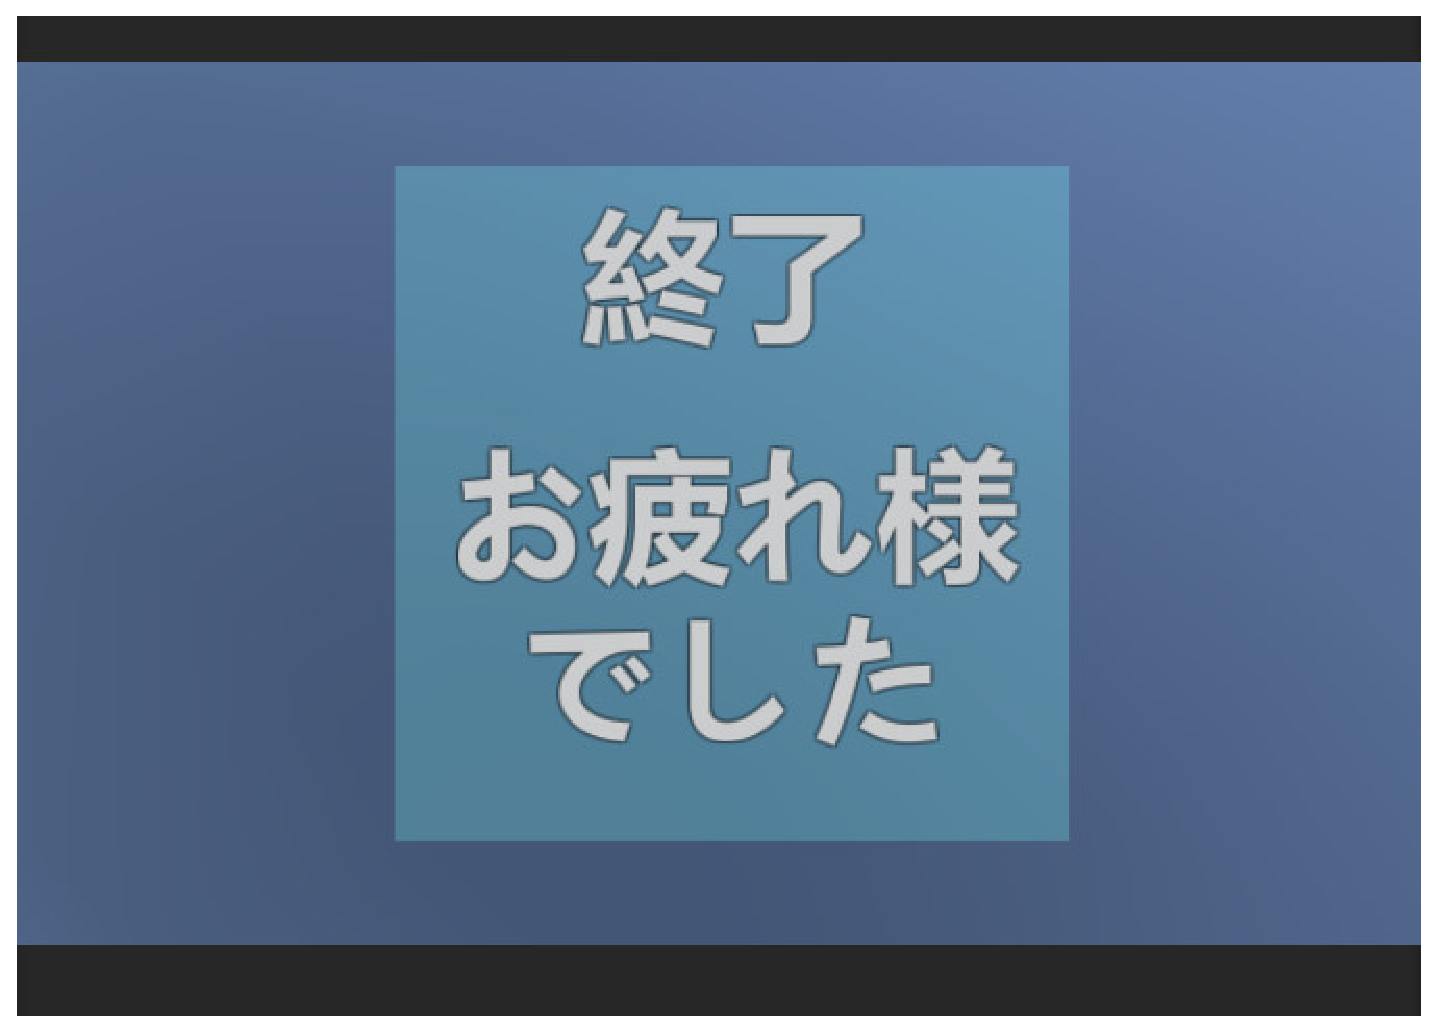
\includegraphics[width=0.9\textwidth]{chap2-figure/end.eps}
	\caption{終了画面}
	\label{fig:end}
\end{figure}
\fi

\if0
\subsection{歩行距離の設定}
CGキャラクタの歩行距離は,ベッド型の下肢リハビリ装置から読み取れる動作周波数から計算され,動作周波数$N$秒間の1周期ごとに,CGキャラクタが$M$m進む.設定した時間までCGキャラクタは歩行動作を続ける.

\subsection{キャラクタの視点設定}
HMDには,センサが内蔵されており,頭部の動きに応じて映像がリアルタイムに追従するので,仮想空間に没入できる利点がある.すなわち,患者が頭部を動かすと,仮想空間内に配置されたCGキャラクタの視点も追従して変わり,HMDの持つ没入感という利点を活かしている.図\ref{fig:geammidstream}に,プレイ途中に頭部を動かした一例を示す.

\begin{figure}[tbp]
	\centering
			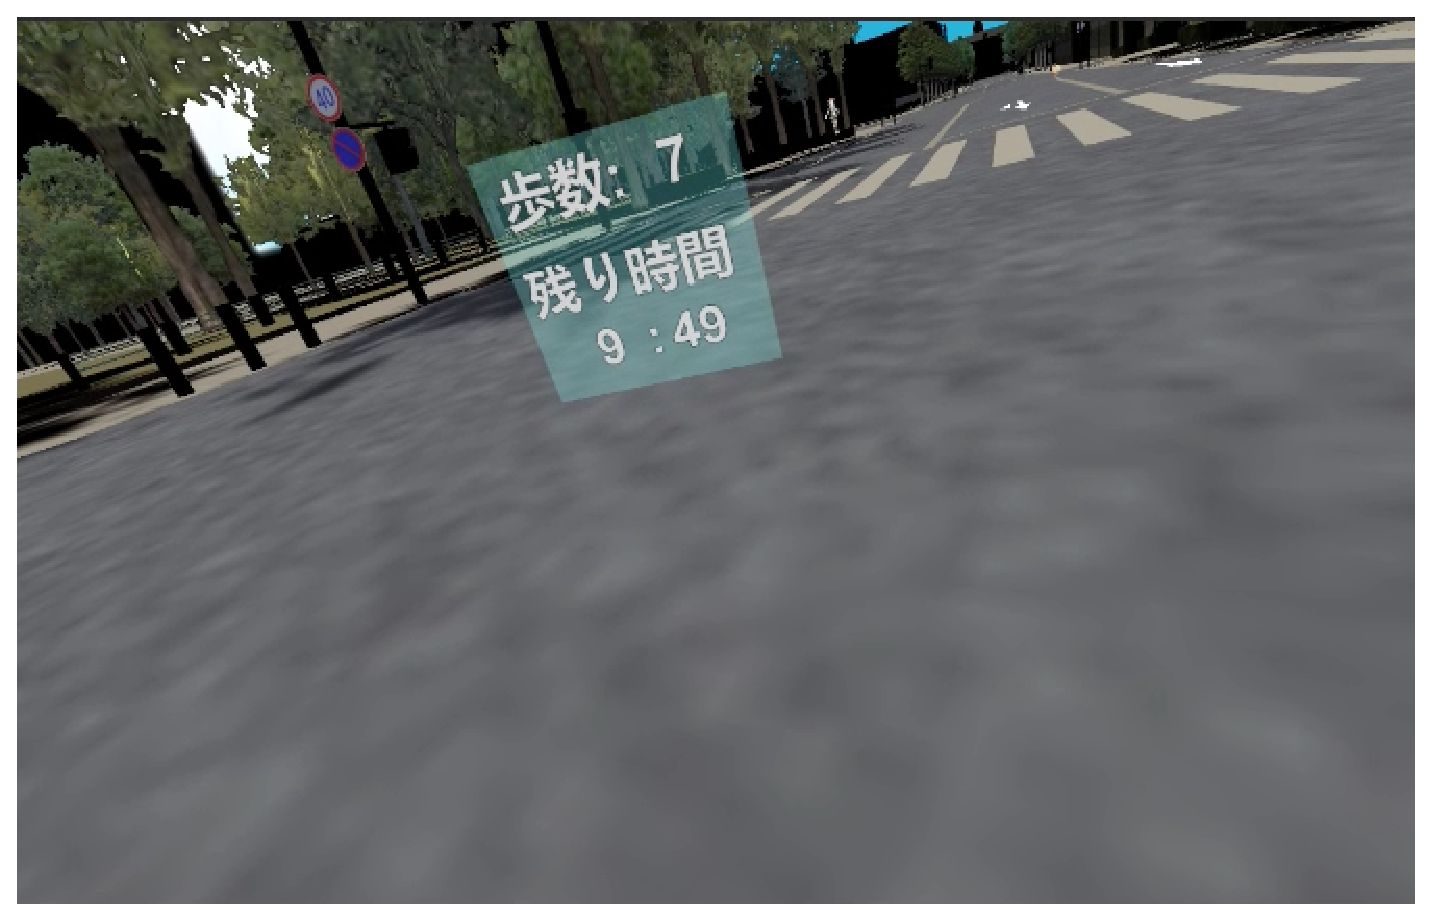
\includegraphics[width=0.9\textwidth]{chap2-figure/midstream-2.eps}
	\caption{プレイ途中視点を変えた図}
	\label{fig:geammidstream}
\end{figure}
\fi

\section{むすび}

\if0
本章では,ベッド型の下肢リハビリ装置から読み取れる動作周波数から計算されるCGキャラクタの歩行距離によって,3D都市モデル空間でのCGキャラクタの移動を行う手法について述べた.ベッド型の他動歩行器と同時に体験するシステムのためのキャラクタの視点の変更を行う手法を記述した.第3章では,大学生の被験者に対して行った提案システムに関するアンケート評価について述べる.
\fi

% Local Variables: 
% mode: japanese-LaTeX
% TeX-master: "root"
% End: 
